%!TEX ROOT=../ctutest.tex

\chapter{Dissertation plan}
\label{chap:plan}


\section{Current research agenda}
\subsection{Automated claim generation}
\todo{}
\subsection{Claim generation metrics}

\begin{figure}
    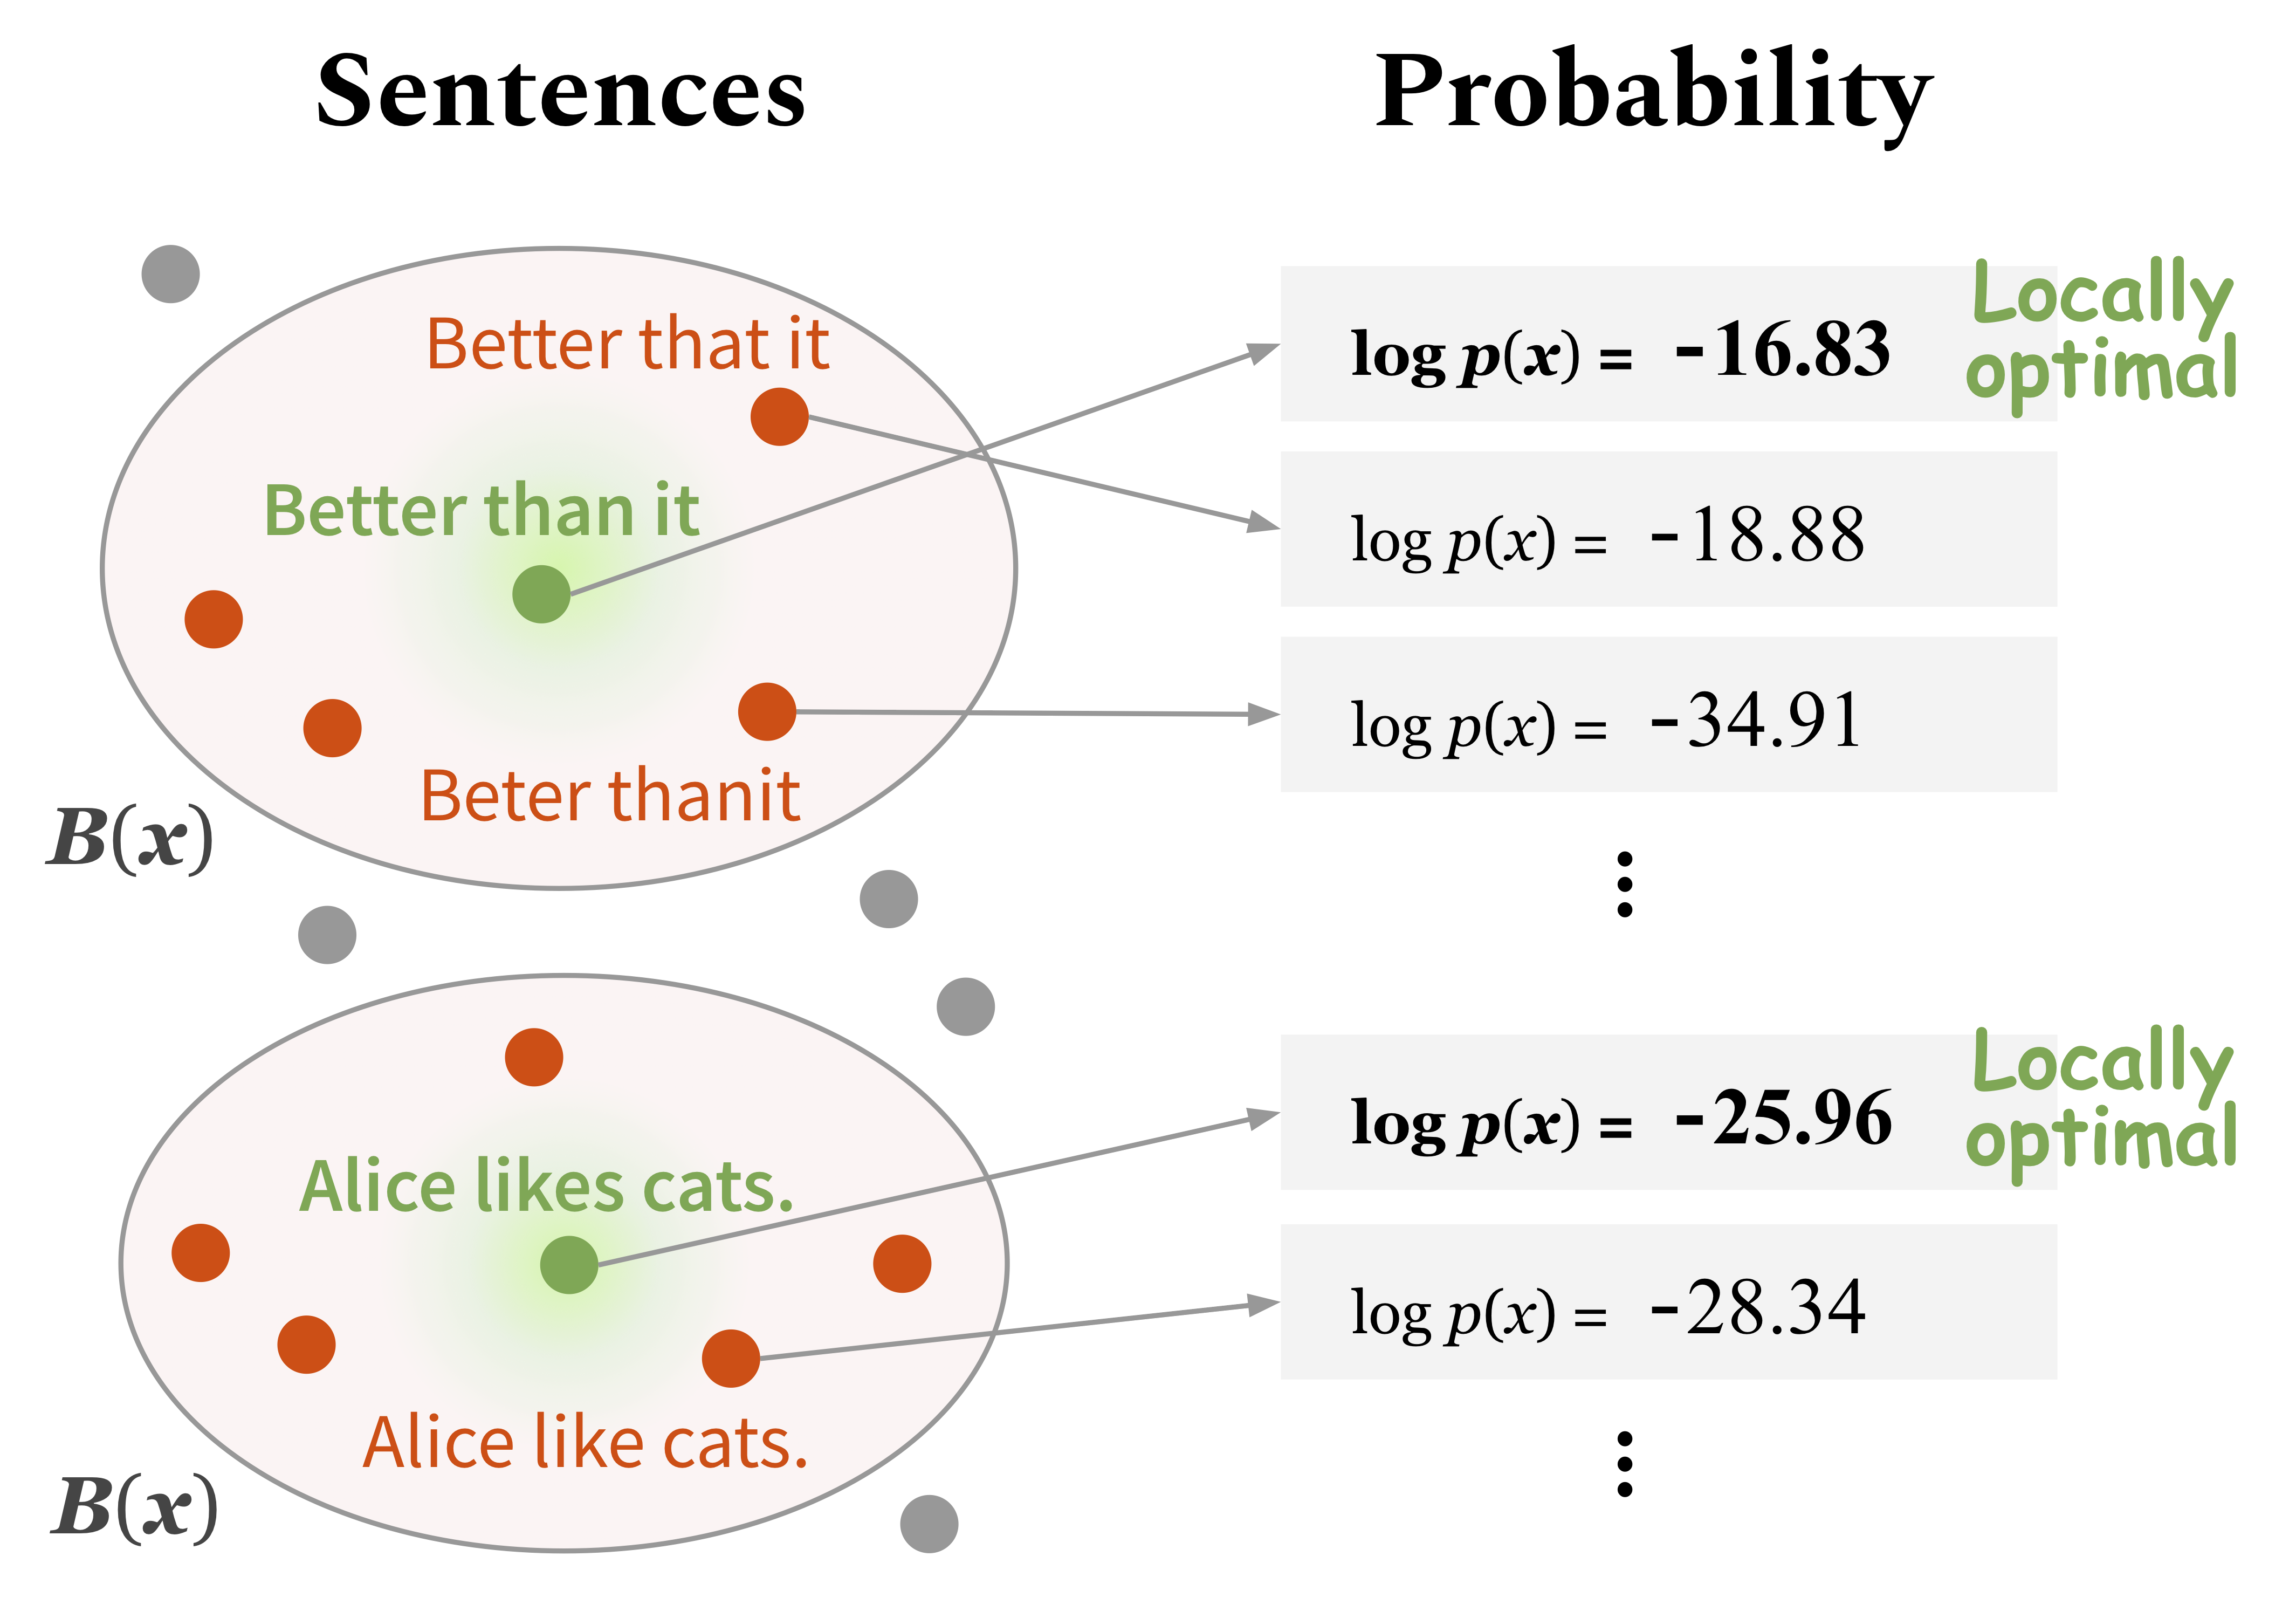
\includegraphics[width=7cm]{fig/lm_critics.png}
    \caption{\textsf{LM-Critic} -- deciding text fluency viewed as finding local optima of Language Model output probability, reprinted from~\cite{yasunaga-etal-2021-lm}}
    \label{fig:lmcritic}
\end{figure}
\label{sec:metrics}

\begin{figure}
    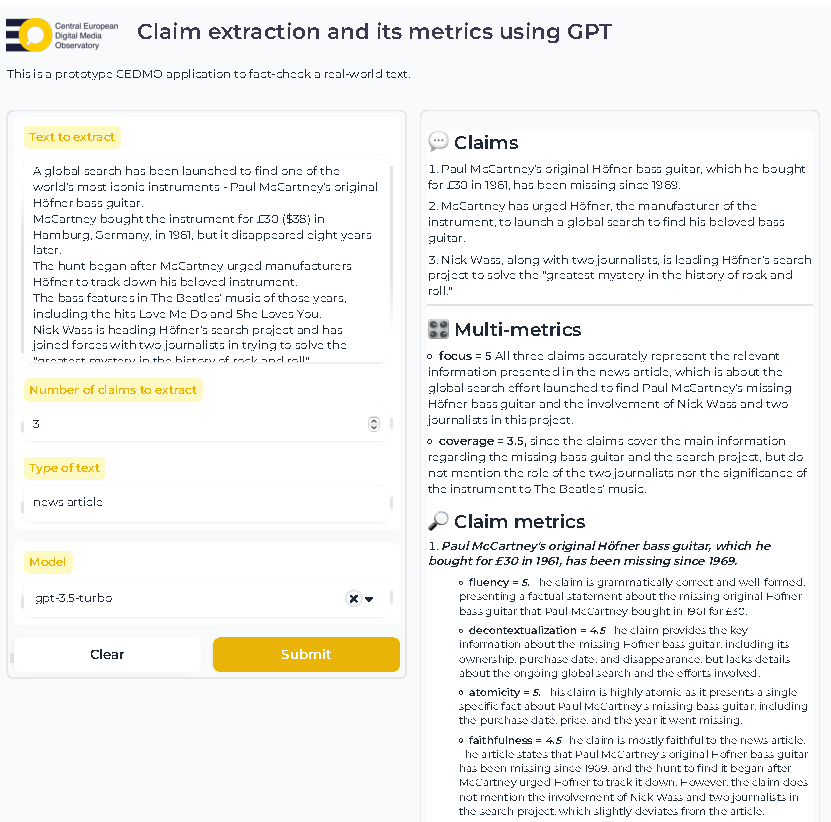
\includegraphics[width=11cm]{fig/gptext.pdf}
    \caption{A self-evaluating claim generation model based on GPT-4~\cite{gpt4} using the \textsf{OpenAI API} and a few-shot approach}
    \label{fig:gptext}
\end{figure}
\label{sec:metrics}
The common problem with generative tasks in NLP is that of explaining model reasoning in human-understandable manner and troubleshooting the prediction faults, such as the \textit{model hallucination}.

For the task of claim generation, where we also face the challenge of the \textit{relevance} of the information extracted by the model, we postulate the following metrics:

\begin{enumerate}
    \item {\techbf Fluency} -- \textit{is the claim grammatically correct and intelligible?}
    
    Currently, we are working with two emulations of claim fluency, challenge that is similar to a standard NLP task of Gramatical Error Detection (GED): \textsf{LM-Critic} (Figure~\ref{fig:lmcritic})~\cite{yasunaga-etal-2021-lm} perturbs the claim words and characters to find local optima in output probability of its tokens, using a language model such as GPT-2 as its reference. \textsf{GPTScore}~\cite{fu2023gptscore} uses prompting a LLM (such as GPT-3.5) to obtain a model-inferred score using few- or zero-shot learning.
    
    Both can be adapted for Czech and the latter is demonstrated in Figure~\ref{fig:gptext}.
    \item {\techbf Decontextualization} -- \textit{can the claim be correctly interpreted without any additional context from the source document or elsewhere?}
    
    A common problem with machine-extracted factual claims is reusing excerpts from source document along with inexplicable contextual pronouns (\"{President won't sue \textit{them}}) and relative referencing (\"{\textit{Last year}, CTU had 23K students}).

\cite{choi-etal-2021-decontextualization} proposes decontextualization as a sequence to sequence task with two texts on input $(s,c)$ -- sentence and context.
    T5 model~\cite{t5-11b} is then trained on machine-generated gold data from Wikipedia to output sentence $s^\prime$ such that the truth-conditional meaning of $s^\prime$ in an empty context is the same as that of $s$ in $c$.

    \cite{mohri2023learning} improves upon this, altering the problem formulation to minimizing surrogate loss, rejecting with a fixed predictor and claiming to get as close as $\sim3\%$ away from the theoretical limit for the task.

    The approaches are reproducible using Czech Wikipedia corpus and appropriate for further examination.

    \item {\techbf Atomicity} --  \textit{does the claim describe a single entity, relation or process?}
    
    can be checked using the Relationship Extraction methods such as LUKE~\cite{yamada2020luke}. To put it simply, the RE task is to identify the entities of a text (persons, institutions,\dots) and the relations between them (such as $(\textit{\"{study at}}, \textit{Herbert}, \textit{CTU})$). The atomicity evaluation can be converted to a RE task by attempting to extract such fact triples and mark the claim as atomic if there is at most one such triple found (after removing symmetries)

    \item {\techbf Faithfulness} -- \textit{does the claim only contain information that is consistent with the source document?}
    
    This metric is crucial to pinpoint \textit{model hallucinations} -- parts of claim where the model outputs stray from the information present in source text and begin to just \"{make stuff up}. We proceed to use two alternative metrics -- a score proposed within the FFCI evaluation framework~\cite{ffci} as: 
    $$\text{AvgTop-}n_{s_j\in X, t_i\in Y^\prime}(\textsc{BERTScore}(t_i,s_j))$$
    Where the $\text{AvgTop-}n$ simply averages across the top $n$ (say, 5) highest scores, $X,Y^\prime$ are the sentences of source document and output (so, in the claim generation scenario $|Y^\prime|=1$) and $\textsc{BERTScore}$~\cite{bert-score} is a recently popular similarity score between two sentences that doesn't compare the texts on a verbatim level (like e.g., ROUGE~\cite{lin-2004-rouge} which correlates poorly with human judgement) but expresses the sentence similarity as a sum of cosine similarities between their tokens' embeddings -- this should capture semantical relations rather than the word-for-word similarity, which could be benefitial in highly inflected languages such as Czech.

    Similar metric called \textsc{AlignScore} was proposed in~\cite{zha2023alignscore}, looking for optimum alignment of output and input parts, in terms of a RoBERTa model~\cite{roberta} trained to detect inconsistencies on 4.7M training examples adapted from various tasks (inference, question answering, paraphrasing,\dots) and while relatively small (355M parameters), outperforms metrics based on GPT-4 that is orders of magnitude larger. 

    Empirically, the models work encouragingly well on spotting hallucinations and inconsistencies in English, and while the transduction of \textsc{BERTScore} is trivial, using a Czech embedding model such as CZERT~\cite{czert} or FERNET~\cite{fernet}, reproducing the success of \textsc{AlignScore} will require more research and data.

    \item {\techbf Focus}$@k$ -- \textit{if we generate $k$ claims using this model, what will be the proportion of gold (relevant) information among all the information listed in the generated claims?}
    
    The metric is analogous to the concept of \textit{precision} in the common machine learning applications, however, its deciding gets more ambiguous in the natural language settings, where we are dealing with synonyms and endless number of possible wordings for every piece of information.

    An ellegant and functional perspective on the problem has been brought around in QAGS\footnote{Pronounced \"{kags}, stands for \"{Question Answering and Generation for Summarization}} evaluation protocol~\cite{wang-etal-2020-asking}, where the idea is to use a Question Generation model (QG) to formulate questions in natural language based on all $k$ predicted claims. The questions are then twice answered using a Question Answering (QA) model, giving it knowledge from (i.) the predicted claims (ii.) the gold claims written by a human.
    The focus is then defined as the proportion of questions with the same answers extracted from the gold and predicted claims, among all questions model can generate from the predicted claims. 

    \item {\techbf Coverage}$@k$ -- \textit{if we generate $k$ claims using this model, what proportion of gold (relevant) information from the source text will be covered?}
    
    Anologous to \textit{recall@k} in general machine learning, QAGS proposes to generate questions using gold claims and try to answer them using the predicted claims, much like in the \textit{focus} scenario, but vice versa.
\end{enumerate}

\section{Data Collection}
\subsection{Human-in-the-loop grading of claim generators}
\subsection{Validation of the model outputs with human fact-checkers}
\subsection{Polish dataset scraping}
Will be first of its kind for NLP purposes

\subsection{Crowd-sourced fact checking platform}
\todo{Cite boys}~\cite{butora}
\section{The grand scope}
\begin{enumerate}
    \item \textbf{Claim extraction metrics proposal based on factuality of summarization}
    \item \textbf{Claim extraction paradigm that benchmarks best in the newly given metrics}
    \item Systems for NLI built on top of LoRA paradigm to score best in the task, as showed promising by Daniil
    
\end{enumerate}